%%%%%%%%%%%%%%%%%%%%%%%%%%%%%%%%%%%%%%%%%%%%%%%%%%%%%%%%%%%%%%%%%%%%%%%%%%%%%%%%%%%%%%
\begin{project}
{Virtual reality data exploration}
{Data immersion - exploring the data in Virtual Reality.} 
{ 
Mobile app (applicable for Oculus Rift):
\begin{itemize}
	\item Reading the data and creating the cloud of points, surfaces etc.
	\item Handling events (e.g. clicking on point to get more detailed meta-data)
\end{itemize}
\begin{center}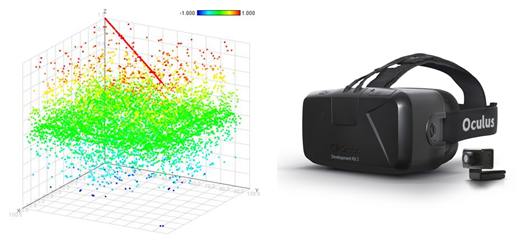
\includegraphics[height=4cm]{oculus.png}\end{center}
}
{-}
{Slawomir Andrzejewski, Krzysztof Wascinski, Krzysztof Wisniowski}
{1 semester}
{2-4}
\end{project}
%%%%%%%%%%%%%%%%%%%%%%%%%%%%%%%%%%%%%%%%%%%%%%%%%%%%%%%%%%%%%%%%%%%%%%%%%%%%%%%%%%%%%%
\begin{project}
{Universal YANG data parser for Cloud Network Element configuration}
{Introduction of Cloud Network Elements support for automated configuration planning.} 
{ 
Create web based tool which enables to import Cloud NE file based configuration and translate it to standarized xls-based format. Cloud NE parametrization is based on YANG model with usage of NETCONF protocol, both open and standarized formats. Solution should provide also export functonality.
\begin{center}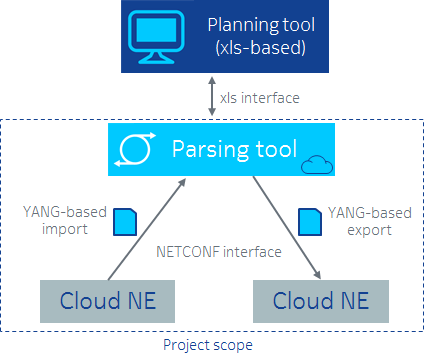
\includegraphics[height=8cm]{yang.png}\end{center}
}
{-}
{Pawel Dmochowski, Mariusz Wegrzyn}
{1 semester}
{2-4}
\end{project}
%%%%%%%%%%%%%%%%%%%%%%%%%%%%%%%%%%%%%%%%%%%%%%%%%%%%%%%%%%%%%%%%%%%%%%%%%%%%%%%%%%%%%%
\begin{project}
{IoT aided planning of urban transport infrastructure}
{IoT aided algorithms for urban transport infrastructure planning.} 
{ 
Looking for correlations for various sources of public data to help planning of urban transport network infrastructure.

\textbf{Inputs:}
\begin{itemize}
	\item Urban bike data WRM/Nextbike, time and place of rental and return, data from the last year
	\item Public transport (MPK) data on vehicles location, historical data from the last year
	\item Urban-scale average speed, public data (korkowo.pl), or data from urban monitoring
	\item Weather reports, publicly available historical data from the last year
	\item GPS logs of users logging their bike routes into the social media, Endomondo, European Cycling Challenge
\end{itemize} 
\textbf{Outputs and analytics:}
\begin{itemize}
	\item Planning of the new cycling routes based on the point of rental and return of the bike
	\item Planning of the new cycling routes based on the route occupation from its  GPS profile on social media
	\item Correlation of urban bike stations with bus stops, opportunities to join both forms of transportation
	\item Mutual dependency between vehicles average speed and number of bikes in use, estimations how much bikes would reduce traffic jam significantly,
	\item Correlation of bikes in use with weather 
\end{itemize} 
}
{-}
{Piotr Grzybowski}
{1 semester}
{2-4}
\end{project}
%%%%%%%%%%%%%%%%%%%%%%%%%%%%%%%%%%%%%%%%%%%%%%%%%%%%%%%%%%%%%%%%%%%%%%%%%%%%%%%%%%%%%%
\begin{project}
{Predicting trends and factors affecting environmental pollution}
{Predicting trends and factors affecting environmental pollution, looking for the main affecting factors and means to restrict them, benchmarking with other agglomerations.} 
{ 
Looking for correlations for various sources of public data to predict the likelihood of growth in air pollution.

\textbf{Inputs:}
\begin{itemize}
	\item Urban-scale average speed, public data (korkowo.pl), or data from urban monitoring
	\item Weather reports, publicly available historical data from the last year
	\item Air pollution data from measuring stations, historical data from the last year
	\item Urban data of the cities studied (size, population, public transport, traffic jams)
	\item Calendar of local festivals and events
\end{itemize} 
\textbf{Outputs and analytics:}
\begin{itemize}
	\item Determine the correlation between air pollution, car traffic and weather conditions, finding trends.
	\item Finding repeating patterns would allow the creation of smog warnings.
	\item Verification of patterns between different towns.
	\item City benchmarking
\end{itemize} 
}
{-}
{Piotr Grzybowski}
{1 semester}
{2-4}
\end{project}
%%%%%%%%%%%%%%%%%%%%%%%%%%%%%%%%%%%%%%%%%%%%%%%%%%%%%%%%%%%%%%%%%%%%%%%%%%%%%%%%%%%%%%
\begin{project}
{LTE network simulator}
{Help novice to understand message flow in cellular network} 
{ 
Create web application visualizing message flow in cellular network. Starting
from one LTE base station and one cell phone visualize what messages are exchanged between them 
in situation like: UE start up, phone call, SMS, web browsing, etc.
}
{At least one team member with telecommunication knowledge.}
{Marek Kukulski}
{1 semester}
{2-5}
\end{project}
%%%%%%%%%%%%%%%%%%%%%%%%%%%%%%%%%%%%%%%%%%%%%%%%%%%%%%%%%%%%%%%%%%%%%%%%%%%%%%%%%%%%%%
\begin{project}
{Handover testing tool based on empirical propagation models}
{The tool will allow to test handovers in more realistic conditions.} 
{ 
Develop tool with GUI interface which on the basis of: base stations locations, antenna heights, transmitting powers, mobile user movement and propagation model (e.g. Free Space, Okumura-Hata) calculates and sets attenuation of multiple programmable attenuator system (e.g. JFW 50PA-847).
}
{Preferred language: Python\newline
At least one team member with telecommunication knowledge.}
{Mariusz Zamlynski}
{1 semester}
{1-5}
\end{project}
%%%%%%%%%%%%%%%%%%%%%%%%%%%%%%%%%%%%%%%%%%%%%%%%%%%%%%%%%%%%%%%%%%%%%%%%%%%%%%%%%%%%%%
\begin{project}
{Lightweight C++11 code model}
{Develop a plugin for Vim or Emacs which uses Clang to provide real-time
syntax highlighting, code completion and error/warning indication} 
{ 
Modern C++ IDEs such as Qt Creator or Microsoft Visual Studio provide code
models for real-time syntactic and semantic code analysis. This greatly enhances 
the programming experience, allowing for faster and more convenient development. 
However, sometimes developers are required to work on remote machines, e.g. via SSH. 
In such circumstances it is impossible to use heavy tools with sophisticated GUIs. 
On the other hand, console text editors do not provide satisfactory code models. 
Existing plugins are often difficult to configure and aimed mainly at graphical versions of the editors. 
They also cause significant problems when new C++11 constructs are used. The growing popularity of Clang,
a modern compiler which supports the full C++11 standard and provides a convenient API, seems to indicate 
the possibility to provide a lightweight plugin for one of the popular console text editors such as Vim or 
Emacs – one that would support real-time syntax highlighting, code completion, compiler error/warning indication. 
 
The plugin will have to be able to:
\begin{itemize}
	\item Load projects, preferably using CMake input files.
	\item Parse the headers and source files belonging to the project as well as
	system libraries to provide a list of available symbols.
	\item Perform on-the-fly code inspection, verifying its syntactic correctness and the symbols used.
	\item Provide real-time information on types of variables, class members and function arguments.
	\item Locate class and function declarations and definitions.
\end{itemize} 
 }
{At least one team member with telecommunication knowledge.}
{Marek Gulanowski}
{1 semester}
{2-5}
\end{project}
%%%%%%%%%%%%%%%%%%%%%%%%%%%%%%%%%%%%%%%%%%%%%%%%%%%%%%%%%%%%%%%%%%%%%%%%%%%%%%%%%%%%%%
\begin{project}
{Competence map}
{Prepare application which allows users to find people with specified experience and create their own competence maps.} 
{
In big company work many people with different experience and competence. The problem is, to find person which has qualification, skills or knowledge, we are looking for at the moment.
Application which can hold map, tags or description of personal abilities will help many people. 
Application should give users such features like:
\begin{itemize}
	\item Ability to traverse through company general abilities map
	\item Ability of create and manage own users map or maps, which can base on company map or its branch
	\item Ability of add, move or remove people from their own competence map
	\item Add, remove competence tags to selected people
	\item Add, remove and edit competence description to selected persons
	\item Ability of search people competence by tags or words in description
	\item Display  the degree if coverage tags with other users data 
	\item User friendly interface for desktops and mobile devices
\end{itemize}
The project will have 3 phases:
\begin{itemize}
	\item Development
	\item Implementation for internal use, without general company map (users can create their own maps, add tags and descriptions)
	\item Development of aggregation tool which help to gain all knowledge about specified people and after that create general company competence map
	\item Implement tool and create such map
\end{itemize}
When user decides that his fellow has some knowledge in some discipline, he add profile of his fellow to his map. User specifies how to tag this knowledge and where he can find this person - also tag with department name or team name.
When user after some time have such problem and doesn't remember how can help, he get in this application and search people with such tags.
}
{-}
{Pawel Gora}
{1 semester}
{3-6}
\end{project}
%%%%%%%%%%%%%%%%%%%%%%%%%%%%%%%%%%%%%%%%%%%%%%%%%%%%%%%%%%%%%%%%%%%%%%%%%%%%%%%%%%%%%%
\begin{project}
{Knowledge-based Expert System simulation environment}
{Ready to use simulation environment with CLIPS production system implemented.}
{
Knowledge-Based Expert System (KBES) is an artificial intelligence branch used for defining human-like reasoning, i.e. decision-making. The goal of the project is to integrate CLIPS system with some simulation environment (e.g. MATLAB), propose the object to be controlled, and define some set of production rules to test, whether it works fine enough. }
{C, C++, MATLAB, CMake, general AI knowledge}
{Pawel Ptasznik}
{1 semester}
{1-2}
\end{project}
%%%%%%%%%%%%%%%%%%%%%%%%%%%%%%%%%%%%%%%%%%%%%%%%%%%%%%%%%%%%%%%%%%%%%%%%%%%%%%%%%%%%%%
\begin{project}
{Nvidia CUDA acceleration for robotic algorithms}
{Our task is to adjust ODE solver, matrix operations, and other necessary components to easily work with both CPU and GPU exploiting theirs full performance.}
{
\textbf{Basic work to be done (list is not exhaustive):}
\begin{itemize}
	\item implement an OdeInt facade
	\item integrate boost::ublas and thrust::device\_vector interfaces
	\item implement (serial) some basic robotic (not necessarily) algorithms
	\item re-implement them in parallel
\end{itemize}
\textbf{During this project you will learn:}
\begin{itemize}
	\item how to use GPU to accelerate your algorithms
	\item how to effectively use your theoretical knowledge in real applications
	\item how to use version control tool (GitHub) and share your work with team
	\item how to use embedded hardware (Nvidia Jetson)
\end{itemize}
\begin{center}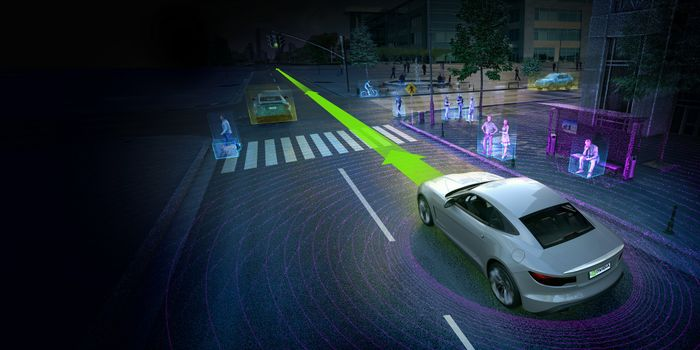
\includegraphics[height=5cm]{automdrive.png}\end{center}
}
{C++ (intermediate level), interest in research in the field of artificial intelligence, control systems and GPU accelerated computing}
{Pawel Ptasznik}
{1 semester}
{1-4}
\end{project}
%%%%%%%%%%%%%%%%%%%%%%%%%%%%%%%%%%%%%%%%%%%%%%%%%%%%%%%%%%%%%%%%%%%%%%%%%%%%%%%%%%%%%%

